\achapter{29}{Inner Products} \label{sec:inner_products}

\vspace*{-17 pt}
\framebox{\hspace*{3 pt}
\parbox{4.7 in}{\begin{fqs}
\item What is an inner product? What is an inner product space?
\item What is an orthogonal set in an inner product space? 
\item What is an orthogonal basis for an inner product space?  
\item How do properties of orthogonality in $R^n$ generalize to orthogonality in an inner product space?
\item How do we find the coordinate vector for a vector in an inner product space relative to an orthogonal basis for the space? 
\item What is the projection of a vector orthogonal to a subspace and why are such orthogonal projections important?
\end{fqs}} \hspace*{3 pt}}

\vspace*{13 pt}

\csection{Application: Fourier Series}

In calculus, a Taylor polynomial for a function $f$ is a polynomial approximation that fits $f$ well around the center of the approximation. For this reason, Taylor polynomials are good \emph{local} approximations, but they are not in general good global approximations. In particular, if a function $f$ has periodic behavior it is impossible to model $f$ well globally with polynomials that have infinite limits at infinity. For these kinds of functions, trigonometric polynomials are better choices. Trigonometric polynomials lead us to Fourier series, and we will investigate how inner products allow us to use trigonometric polynomials to model musical tones later in this section. 


\csection{Introduction}

We have seen that orthogonality in $\R^n$ is an important concept. We can extend the idea of orthogonality, as well as the notions of length and angles, to a variety of different vector spaces beyond just $\R^n$ as long as we have a product like a dot product. Such products are called \emph{inner products}. Inner products lead us to many important ideas like Fourier series, wavelets, and others.

Recall that the dot product on $\R^n$ assigns to each pair of vectors $\vu$ and $\vv$ the scalar $\vu \cdot \vv$. Thus, the dot product defines a mapping from $\R^n \times \R^n$ to $\R$. Recall also that the dot product is commutative, distributes over vector addition, and respects scalar multiplication. Additionally, the dot product of a vector by itself is always non-negative and is equal to 0 only when the vector is the zero vector. There is nothing special about using $\R^n$ as the source for our vectors, and we can extend the notion of a dot product to any vector space using these properties. 

\begin{definition} \label{def:6_c_inner_product}  An \textbf{inner product}\index{inner product} $\langle \ , \ \rangle$ on a vector space $V$ is a mapping from $V \times V \to \R$ satisfying
\begin{enumerate}
\item $\langle \vu , \vv \rangle = \langle \vv , \vu \rangle$ for all $\vu$ and $\vv$ in $V$,
\item $\langle \vu + \vv , \vw \rangle = \langle \vu , \vw \rangle + \langle \vv , \vw \rangle$ for all $\vu$, $\vv$, and $\vw$ in $V$,
\item $\langle c\vu , \vv \rangle = c\langle \vu , \vv \rangle$ for all $\vu$, $\vv$ in $V$ and all scalars $c$,
\item $\langle \vu , \vu \rangle \geq 0$ for all $\vu$ in $V$ and $\langle \vu , \vu \rangle = 0$ if and only if $\vu = \vzero$.
\end{enumerate}
An \textbf{inner product space}\index{inner product space} is a vector space on which an inner product is defined.
\end{definition} 


\begin{pa} \label{pa:6_c} ~
\be
\item Suppose we are given the mapping from $\R^2 \times \R^2$ to $\R$ defined by
\[\langle \vu, \vv \rangle = u_1v_1 + 2u_2v_2\]
for $\vu = [u_1 \ u_2]^{\tr}$ and $\vv = [v_1 \ v_2]^{\tr}$ in $\R^2$. Check that this mapping satisfies all of the properties of an inner product.  \item 

\item Now consider the mapping from $\R^2 \times \R^2$ to $\R$ defined by 
\[\langle \vu, \vv \rangle = 2u_1v_1 - 3u_2v_2\]
for $\vu = [u_1 \ u_2]^{\tr}$ and $\vv = [v_1 \ v_2]^{\tr}$ in $\R^2$. Show that this mapping does not satisfy the fourth property of an inner product. 

\item Finally, show that the mapping from $\pol_1 \times \pol_1 \to \R$ defined by 
\[\langle a_0+a_1t, b_0+b_1t \rangle = a_0b_0 + a_1b_1\]
 for $a_0+a_1t, b_0+b_1t$ in $\pol_1$ is an inner product on $\pol_1$. 

\ee

\end{pa}

%\begin{pa}
%\be
%\item Use the definition of an inner product to determine which of the following defines an inner product on the indicated space. Verify your answers.
%    \ba
%    \item $\langle \vu, \vv \rangle = u_1v_1 + 2u_2v_2$ for $\vu = [u_1 \ u_2]^{\tr}$ and $\vv = [v_1 \ v_2]^{\tr}$ in $\R^2$


%    \item $\langle \vu, \vv \rangle = 2u_1v_1 - 3u_2v_2$ for $\vu = [u_1 \ u_2]^{\tr}$ and $\vv = [v_1 \ v_2]^{\tr}$ in $\R^2$


%    \item $\langle a_0+a_1t, b_0+b_1t \rangle = a_0b_0 + a_1b_1$ for $a_0+a_1t, b_0+b_1t$ in $\pol_1$


%    \ea
%How about something like:
%a) Suppose we are given the mapping <u,v>=u1v1+2u2v2 from R^2xR^2->R. Check that this mapping satisfies the properties of an inner product and hence is a valid inner product.
%b) Suppose we are given <u,v> ... . Show that this mapping fails property 4.
%(I'd probably remove c but we can keep it and turn it into a similar form as above.)

%\ee

%\end{pa}

 
\csection{Inner Product Spaces}

As we saw in Definition \ref{def:6_c_inner_product}, the idea of the dot product in $\R^n$ can be extended to define inner products on different types of vector spaces. Preview Activity \ref{pa:6_c} provides two examples of inner products. The examples below provide some important inner products on vector spaces. Verification of the following as inner products is left to the exercises. 

\begin{itemize}
\item If $a_1$, $a_2$, $\ldots$, $a_n$ are positive scalars, then 
\[\langle [u_1 \ u_2 \ \cdots \ u_n]^{\tr},  [v_1 \ v_2 \ \cdots \ v_n]^{\tr} \rangle = a_1u_1v_1+a_2u_2v_2+ \cdots + a_nu_nv_n\]
 defines an inner product on $\R^n$. 
\item Every invertible $n \times n$ matrix $A$ defines an inner product on $\R^n$ by  
\[\langle \vu, \vv \rangle = (A\vu) \cdot (A\vv).\]
\item The definite integral defines an inner product: 
\[\langle f, g \rangle = \int_a^b f(x)g(x) \ dx\]
for $f,g \in C[a,b]$ (where $C[a,b]$ is the vector space of all continuous functions on the interval $[a,b]$ -- that $C[a,b]$ is a vector space is left for Exercise \ref{ex:6_c_Cab})
\item We can use the trace of a matrix (see Definition \ref{def:trace}) to define an inner product on matrix spaces. If $A$ and $B$ are in the space $\M_{n \times n}$ of $n \times n$ matrices with real entries, we define the product $\langle A , B \rangle$ as 
\[\langle A, B \rangle = \trace\left(AB^{\tr}\right).\]
This defines an inner inner product on the space $\M_{n \times n}$ called the \emph{Frobenius} inner product. 
\end{itemize}

Since we defined inner products using the properties of the dot product, we might wonder if inner products actually satisfy all of the other properties of the dot product. For example, $\vu \cdot \vzero = 0$ for any vector $\vu$ in $\R^n$; but is it true that $\langle \vu, \vzero \rangle = 0$ in every inner product space? This property is not part of the definition of an inner product, so we need to verify it if true. 


\begin{activity} \label{act:6_c_ip_zero} Let $\vu$ be a vector in an inner product space $V$. 
    \ba
    \item Why is $\langle \vu, \vzero \rangle = \langle \vu, \vzero \rangle + \langle \vu, \vzero \rangle$?

    

    \item How does the equation in part (a) show that $\langle \vu, \vzero \rangle = 0$?

    

    \ea
\end{activity}

Activity \ref{act:6_c_ip_zero} suggests that inner products share the defining properties of the dot product. Some properties of the inner product are given in the following theorem (the proofs of the remaining parts are left to the Exercises).

\begin{theorem} \label{thm:6_c_inner_product_properties} Let $\langle \ , \ \rangle$ be an inner product on a vector space $V$ and let $\vu, \vv$, and $\vw$ be vectors in $V$ and $c$ a scalar. Then
\begin{enumerate}
	\item $\langle \vzero , \vv \rangle = \langle \vv , \vzero \rangle = 0$
	\item $\langle \vu , c\vv \rangle = c\langle \vu , \vv \rangle$
	\item $\langle \vu , \vv+\vw \rangle = \langle \vu , \vv \rangle + \langle \vu , \vw \rangle$
\item $\langle \vu - \vv, \vw \rangle = \langle \vu , \vw \rangle - \langle \vv , \vw \rangle$
\end{enumerate}
\end{theorem}

Inner products will allow us to extend ideas of orthogonality, lengths of vectors, and angles between vectors to any inner product space.  

\csection{The Length of a Vector}

We can use inner products to define the length of any vector in an inner product space and the distance between two vectors in an inner product space. The idea comes right from the relationship between lengths of vectors in $\R^n$ and the dot product (compare to Definition \ref{def:6_a_length_Rn}). 

\begin{definition} Let $\vv$ be a vector in an inner product space $V$. The \textbf{length}\index{length of a vector in an inner product space} of $\vv$ is the real number
\[||\vv|| = \sqrt{\langle \vv, \vv \rangle}.\]
\end{definition}

The length of a vector in a vector space is also called \emph{magnitude} or \emph{norm}. Just as in $\R^n$ we can use the notion of length to define unit vectors in inner product spaces (compare to Definition \ref{def:6_a_unit_vector}).  

\begin{definition} A vector $\vv$ in inner product space is a \textbf{unit vector}\index{unit vector in an inner product space} if $||\vv|| = 1$.
\end{definition}

We can find a unit vector in the direction of a nonzero vector $\vv$ in an inner product space $V$ by dividing by the norm of the vector. That is, the vector $\ds \frac{\vv}{||\vv||}$ is a unit vector in the direction of the vector $\vv$, provided that $\vv$ is not zero. 

We define the distance between vectors $\vu$ and $\vv$ in an inner product space $V$ in the same way we defined distance in $\R^n$ (compare to Definition \ref{def:6_a_distance}).

\begin{definition} Let $\vu$ and $\vv$ be vectors in an inner product space $V$. The \textbf{distance between}\index{distance between vectors in an inner product space} $\vu$ and $\vv$ is the length of the difference $\vu - \vv$ or
\[|| \vu - \vv ||.\]
\end{definition}


\begin{activity} Find the indicated length or distance in the inner product space.
	\ba
	\item Find the length of the vectors $\vu = [1 \ 3]^{\tr}$ and $\vv=[3 \ 1]^\tr$ using the inner product 
\[\langle [u_1 \ u_2]^{\tr}, [v_1 \ v_2]^{\tr} \rangle = 2u_1v_1 + 3u_2v_2\]
 in $\R^2$.
	
	
	
	\item Find the distance between the polynomials $p(t) = t+1$ and $q(t) = t^2-1$ in $C[0,1]$ using the inner product $\langle f, g \rangle = \int_0^1 f(x)g(x) \ dx$. (You may assume that $\langle \ , \ \rangle$ defines an inner product on $C[0,1]$, the space of continuous functions defined on the interval $[0,1]$.  


	
	\ea
\end{activity}




\csection{Orthogonality in Inner Product Spaces}

We defined orthogonality in $\R^n$ using the dot product (see Definition \ref{def:6_a_orthogonal_dot_product}) and the angle between vectors in $\R^n$. We can extend that idea to any inner product space. 

We can define the angle between two vectors in an inner product space just as we did in $\R^n$. If $\vu$ and $\vv$ are nonzero vectors in an inner product space $V$, then the \textbf{angle} $\theta$ \textbf{between}\index{angle between vectors} $\vu$ \textbf{and} $\vv$ is such that 
\[\cos(\theta) = \frac{|\langle \vu, \vv \rangle|}{||\vu||\, ||\vv||}.\]
and $0\leq \theta \leq \pi$. This angle is well-defined due to the Cauchy-Schwarz inequality $|\langle \vu, \vv \rangle| \leq ||\vu||\, ||\vv||$ whose proof is left to the exercises.

With the angle between vectors in mind, we can define orthogonal vectors in an inner product space. 

\begin{definition} Vectors $\vu$ and $\vv$ in an inner product space $V$ are \textbf{orthogonal}\index{orthogonal vectors in inner product spaces} if
\[\langle \vu, \vv \rangle = 0.\]
\end{definition}
 
Note that this defines the zero vector to be orthogonal to every vector.

\begin{activity} ~
	\ba
	\item Find a nonzero vector in $\R^2$ orthogonal to the vector $\vu = [3 \ 1]^{\tr}$ using the inner product $\langle [u_1 \ u_2]^{\tr}, [v_1 \ v_2]^{\tr} \rangle = 2u_1v_1 + 3u_2v_2$.
	
	
	
		\item Determine if the vector $\vv = \left[ \begin{array}{r} 0\\3\\-2 \end{array} \right]$ is orthogonal to the vector $\vw = \left[ \begin{array}{r} -1\\0\\1 \end{array} \right]$ using the inner product $\langle \vu, \vv \rangle = (A\vu) \cdot (A\vv)$ on $\R^3$, where $A = \left[ \begin{array}{ccc} 0&1&1\\1&1&0\\0&1&0 \end{array} \right]$.
	
	\item Find the angle between the two polynomials $p(t)=1$ and $q(t)=t$ in $\pol_1$ with inner product $\langle r(t),s(t) \rangle = \int_0^1 r(t)s(t) \ dt$.  	

	\ea
\end{activity}

Using orthogonality we can generalize the notions of orthogonal sets and bases, orthonormal bases and orthogonal complements we defined in $\R^n$ to all inner product spaces in a natural way.


\csection{Orthogonal and Orthonormal Bases in Inner Product Spaces}

As we did in $\R^n$, we define an orthogonal set to be one in which all of the vectors in the set are orthogonal to each other  (compare to Definition \ref{def:6_b_orthogonal_set_Rn}).

\begin{definition} A subset $S$ of an inner product space $V$ for which $\langle \vu, \vv \rangle = 0$ for all $\vu \neq \vv$ in $S$ is called an \textbf{orthogonal set}\index{orthogonal set in an inner product space}. 
\end{definition}

As in $\R^n$, an orthogonal set of nonzero vectors is always linearly independent. The proof is similar to that of Theorem  \ref{thm:6_b_Orth_li} and is left to the Exercises. 

\begin{theorem} \label{thm:6_c_Orth_li_ips} Let $\{\vv_1, \vv_2, \ldots, \vv_m\}$ be a set of nonzero orthogonal vectors in an inner product space $V$. Then the vectors $\vv_1$, $\vv_2$, $\ldots$, $\vv_m$ are linearly independent.
\end{theorem}


A basis that is also an orthogonal set is given a special name (compare to Definition \ref{def:6_b_orthogonal_basis_Rn}).

\begin{definition} An \textbf{orthogonal basis}\index{orthogonal basis in an inner product space} $\CB$ for a subspace $W$ of an inner product space $V$ is a basis of $W$ that is also an orthogonal set.
\end{definition}

Using the dot product in $\R^n$, we saw that the representation of a vector as a linear combination of vectors in an orthogonal or orthonormal basis was quite elegant. The same is true in any inner product space. To see this, let $\CB = \{\vv_1, \vv_2, \ldots, \vv_m\}$ be an orthogonal basis for a subspace $W$ of an inner product space $V$ and let $\vx$ be any vector in $W$. We know that
\[\vx = x_1\vv_1 + x_2\vv_2 + \cdots + x_m \vv_m\]
for some scalars $x_1$, $x_2$, $\ldots$, $x_m$. If $1\leq k\leq m$, then, using inner product properties and the orthogonality of the vectors $\vv_i$, we have
\[\langle \vv_k, \vx \rangle = x_1 \langle \vv_k, \vv_1 \rangle + x_2 \langle \vv_k, \vv_2 \rangle + \cdots + x_m \langle \vv_k, \vv_m \rangle = x_k \langle \vv_k, \vv_k \rangle.\]
So
\[x_k = \ds \frac{\langle \vx, \vv_k \rangle}{\langle \vv_k,  \vv_k \rangle}.\]
Thus, we can calculate each weight individually with two simple inner product calculations. 

In other words, the coordinate vector $[\vx]_{\CB}$ of $\vx$ in an inner product space $V$ with orthogonal basis $\CB = \{\vv_1, \vv_2, \ldots, \vv_m\}$ is given by 
\[[\vx]_{\CB} = \left[ \begin{array}{c} \frac{\langle \vx, \vv_1 \rangle}{\langle \vv_1, \vv_1 \rangle} \\ \frac{\langle \vx, \vv_2 \rangle}{\langle \vv_2, \vv_2 \rangle} \\ \vdots \\ \frac{\langle \vx, \vv_m \rangle}{\langle \vv_m, \vv_m \rangle} \end{array} \right].\]
We summarize this discussion in the next theorem (compare to Theorem \ref{thm:6_b_orth_dcomp}).

\begin{theorem} \label{thm:6_c_orth_dcomp} Let $\CB = \{\vv_1, \vv_2, \ldots, \vv_m\}$ be an orthogonal basis for a subspace of an inner product space $V$. Let $\vx$ be a vector in $W$. Then
\begin{equation}
\vx = \ds \frac{\langle \vx, \vv_1 \rangle}{\langle \vv_1, \vv_1 \rangle} \vv_1 +  \frac{\langle \vx, \vv_2 \rangle}{\langle \vv_2, \vv_2 \rangle} \vv_2 + \cdots + \frac{\langle \vx, \vv_m \rangle}{\langle \vv_m, \vv_m \rangle} \vv_m. \label{eq:6_c_orth_decomp_ips}
\end{equation}
\end{theorem}



\begin{activity} Let $p_1(t) = 1-t$, $p_2(t) = -2+4t+4t^2$, and $p_3(t) = 7-41t+40t^2$ be vectors in the inner product space $\pol_2$ with inner product defined by $\langle p(t), q(t) \rangle = \int_0^1 p(t)q(t) \ dt$. Let $\CB = \{p_1(t), p_2(t), p_3(t)\}$. You may assume that $\CB$ is an orthogonal basis for $\pol_2$. Let $z(t) = 4-2t^2$. Find the weight $x_3$ so that $z(t) = x_1p_1(t) + x_2 p_2(t) + x_3 p_3(t)$. Use technology as appropriate to evaluate any integrals. 
%	\ba
%	\item Show that $p_1(t)$ and $p_2(t)$ are orthogonal. (Use the fact that $(1-t)(-2+4t+4t^2) = -2+6t-4t^3$.)


%	\item The set $\CB$ is an orthogonal basis for $\pol_2$ (you may assume this). Let $z(t) = 4-2t^2$. Find the weight $x_3$ so that $z(t) = x_1p_1(t) + x_2 p_2(t) + x_3 p_3(t)$. (Hint: $\int_0^1 (4-2t^2)(7-41t+40t^2) \, dt = -\frac{5}{6}$ and $\int_0^1 (7-41t+40t^2)^2 \, dt = 9$.)

%	\ea
\end{activity}


The decomposition (\ref{eq:6_c_orth_decomp_ips}) is even simpler if $\langle \vv_k, \vv_k \rangle = 1$ for each $k$. Recall that
\[\langle \vv, \vv \rangle = || \vv ||^2,\]
so the condition $\langle \vv, \vv \rangle  = 1$ implies that the vector $\vv$ has norm 1. As in $\R^n$, an orthogonal basis with this additional condition is given a special name (compare to Definition \ref{def:6_b_orthonormal_basis}).

\begin{definition} An \textbf{orthonormal basis}\index{orthonormal basis in an inner product space} $\CB = \{\vv_1, \vv_2, \ldots, \vv_m\}$ for a subspace $W$ of an inner product space $V$ is an orthogonal basis such that $|| \vv_k || = 1$ for $1\leq k\leq m$.
\end{definition}

If $\CB = \{\vv_1, \vv_2, \ldots, \vv_m\}$ is an orthonormal basis for a subspace $W$ of an inner product space $V$ and $\vx$ is a vector in $W$, then  (\ref{eq:6_c_orth_decomp_ips}) becomes
\begin{equation}
\vx = \langle \vx, \vv_1 \rangle \vv_1 +  \langle \vx, \vv_2 \rangle \vv_2 + \cdots + \langle \vx, \vv_m \rangle \vv_m. \label{eq:6_c_orthnorm_decomp_ips}
\end{equation}

A good question to ask here is how we can construct an orthonormal basis from an orthogonal basis.



\begin{activity} \label{act:6_c_orthon_basis} Consider vectors from an inner product space $V$.
	\ba
	\item Let $\vv_1$ and $\vv_2$ be orthogonal vectors. Explain how we can obtain unit vectors $\vu_1$ in the direction of $\vv_1$ and $\vu_2$ in the direction of $\vv_2$.
	
	
	
	\item Show that $\vu_1$ and $\vu_2$ from the previous part are orthogonal vectors.
	
	
	
	\item Use the ideas from this problem to construct an orthonormal basis for the subspace
\[W = \Span\left\{\left[ \begin{array}{c} 1 \\ 1 \\ 1 \\ 0 \end{array} \right], \left[ \begin{array}{r} -1 \\ 1 \\ -1 \\ 2\end{array} \right], \left[ \begin{array}{r} 8 \\ 5 \\ -31 \\ -3 \end{array} \right]\right\}\]
of the inner product space $\R^4$ with inner product 
\[\langle [u_1 \ u_2 \ u_3 \ u_4]^\tr, [v_1 \ v_2 \ v_3 \ v_4]^\tr \rangle = 2u_1v_1+3u_2v_2+u_3v_3+5u_4v_4.\]
(Note that you need to check for orthogonality.)	
	
	
	\ea
\end{activity}

\csection{Orthogonal Projections onto Subspaces}

\begin{pa} \label{pa:6_c_2} Let $\CB = \{\vw_1, \vw_2\}$ be a basis for a subspace $W$ of $\R^3$,  where $\vw_1 = [1 \ 0 \ 0]^{\tr}$ and $\vw_2 = [0 \ 1 \ 0]^{\tr}$. Note that $\CB$ is an orthonormal basis for $W$ using the dot product as inner product. Let $\vv = [1 \ 2 \ 1]^{\tr}$. Notice also that $W$ is the $xy$-plane and that $\vv$ is not in $W$ as illustrated in Figure \ref{F:6_d_o_proj}.
	\be
	\item Find the orthogonal projection $\vu_1$ of $\vv$ onto $W_1 = \Span\{\vw_1\}$. (Hint: See Equation (\ref{eq:6_a_projection}).) 

	
	\item Find the orthogonal projection $\vu_2$ of $\vv$ onto $W_2 = \Span\{\vw_2\}$.

	\item Calculate the distance between $\vv$ and $\vu_1$ and $\vv$ and $\vu_2$. Which of $\vu_1$ and $\vu_2$ is closer to $\vv$?
			
	\item Show that the vector $\frac{1}{2} [1 \ 4 \ 0]^{\tr}$ is in $W$ and find the distance between $\vv$ and $\frac{1}{2} [1 \ 4 \ 0]^{\tr}$.

\item Part (4) shows that neither vector $\vu_1 = \proj_{\vw_1} \vv$ nor $\vu_2 = \proj_{\vw_2} \vv$ is the vector in $W$ that is closest to $\vv$. We should probably expect this since neither projection uses the fact that the other vector might contribute to the closest vector. Our goal is to find the linear combination $\vw$ of $\vw_1$ and $\vw_2$ in $W$ that makes $|| \vw - \vv ||$ the smallest. Letting $\vw = a \vw_1 + b\vw_2$, we have that $||\vw - \vv|| = \sqrt{(a-1)^2 + (b-2)^2 + 1}$. Find the weights $a$ and $b$ that minimize this norm $||\vw - \vv||$. 
	
\item A picture of $\vw_1$, $\vw_2$, $W$, and $\vv$ is shown in Figure \ref{F:6_d_o_proj}. Draw in $\vu_1$, $\vu_2$, and the vector $\vw$ you found in part (5). There is a specific relationship between this vector $\vw$ and $\vu_1$ and $\vu_2$. Describe this relationship algebraically and illustrate it graphically in Figure \ref{F:6_d_o_proj}.  
\begin{figure}[h]
\begin{center}
\resizebox{!}{2.5in}{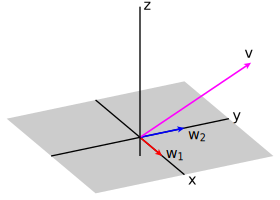
\includegraphics{6_d_O_proj}}
\end{center}
\caption{The space $W$ and vectors $\vw_1$, $\vw_2$, and $\vv$}
\label{F:6_d_o_proj}
\end{figure}


	\ee
\end{pa}


Preview Activity \ref{pa:6_c_2} gives an indication of how we can project a vector $\vv$ in $\R^n$ onto a subspace $W$ of $\R^n$. If we have an orthogonal basis for $W$, we can just add the orthogonal projections of $\vv$ onto each basis vector. The resulting vector is called the orthogonal projection of $\vv$ onto the subspace $W$. As we did with orthogonal projections onto vectors, we can also define the projection of $\vv$ orthogonal to $W$. All of this can be done in the context of inner product spaces. Note that to make this all work out properly, we will need an orthogonal basis for $W$. 

\begin{definition} Let $W$ be a subspace of an inner product space $V$ and let $\CB = \{\vw_1, \vw_2, \ldots, \vw_m\}$ be an orthogonal basis for $W$. For a vector $\vv$ in $V$, the \textbf{orthogonal projection of $\vv$ onto $W$}\index{orthogonal projection onto a subspace} is the vector
\[\proj_W \vv =  \frac{\langle \vv, \vw_1 \rangle }{\langle \vw_1, \vw_1 \rangle } \vw_1 + \frac{\langle \vv, \vw_2 \rangle }{\langle \vw_2, \vw_2 \rangle }  \vw_2 + \cdots + \frac{\langle \vv, \vw_m \rangle}{\langle \vw_m, \vw_m \rangle} \vw_m.\] 
The \textbf{projection of $\vv$ orthogonal to $W$}\index{projection orthogonal to a subspace} is the vector
\[\proj_{W^{\perp}} \vv = \vv - \proj_W \vv.\]
\end{definition}


The notation $\proj_{W^{\perp}} \vv$ indicates that we expect this vector to be orthogonal to every vector in $W$. 

\begin{activity} \label{act:6_c_orth_projection} Let $W = \Span\{\vw_1, \vw_2,\vw_3\}$ in $\R^4$, where $\vw_1 = \left[ \begin{array}{c} 1 \\ 1 \\ 1 \\ 0 \end{array} \right]$, $\vw_2 = \left[ \begin{array}{r} -1 \\ 1 \\ -1 \\ 2\end{array} \right]$, and $\vw_3 =  \left[ \begin{array}{r} 8 \\ 5 \\ -31 \\ -3 \end{array} \right]$. Recall that we showed in Activity \ref{act:6_c_orthon_basis} that this was an orthogonal basis. Find the projection of the vector $\vv = \left[ \begin{array}{c} 2 \\0 \\ 0 \\ 1 \end{array} \right]$ onto $W$ using the inner product 
\[\langle [u_1 \ u_2 \ u_3 \ u_4]^{\tr}, [v_1 \ v_2 \ v_3 \ v_4]^{\tr} \rangle = 2u_1v_1+3u_2v_2+u_3v_3+5u_4v_4.\]
Show directly that $\proj_{W^{\perp}} \vv$ is orthogonal to the basis vectors for $W$.

%	\ba
%	\item Let $W = \Span \{\vw_1, \vw_2\}$ in $\R^3$, with $\vw_1=[1 \ 0 \ 0]^{\tr}$ and $\vw_2= [0 \ 1 \ 0]^{\tr}$,  and  $\vv = [1 \ 2 \ 1]^{\tr}$ as in Preview Activity \ref{pa:6_c_2}. Recall that $\proj_W \vv =  [1 \ 2 \ 0]^{\tr}$. Find the projection of $\vv$ orthogonal to $W$ and show directly that $\proj_{W^{\perp}} \vv$ is orthogonal to the basis vectors for $W$ (and hence to every vector in $W$).
    

%	\item Let $\vw_1 = \left[ \begin{array}{c} 1 \\ 1 \\ 1 \\ 0 \end{array} \right]$, $\vw_2 = \left[ \begin{array}{r} -1 \\ 1 \\ -1 \\ 2\end{array} \right]$, and $\vw_3 =  \left[ \begin{array}{r} 8 \\ 5 \\ -31 \\ -3 \end{array} \right]$, and let $W = \Span\{\vw_1, \vw_2,\vw_3\}$ in $\R^4$. Recall that we showed in Activity \ref{act:6_c_orthon_basis} that this was an orthogonal basis. Find the projection of the vector $\vv = \left[ \begin{array}{c} 2 \\0 \\ 0 \\ 1 \end{array} \right]$ onto $W$ using the inner product 
%\[\langle [u_1 \ u_2 \ u_3 \ u_4]^{\tr}, [v_1 \ v_2 \ v_3 \ v_4]^{\tr} \rangle = 2u_1v_1+3u_2v_2+u_3v_3+5u_4v_4.\]
%Show directly that $\proj_{W^{\perp}} \vv$ is orthogonal to the basis vectors for $W$.
	
%	\ea


\end{activity}

Activity \ref{act:6_c_orth_projection} indicates that the vector $\proj_{W^{\perp}} \vv$ is in fact orthogonal to every vector in $W$. To see that this is true in general, let $\CB = \{\vw_1, \vw_2, \ldots, \vw_m\}$ be an orthogonal basis for a subspace $W$ of an inner product space $V$ and let $\vv$ be a vector in $V$. Let 
\[\vw =  \proj_W \vv = \frac{\langle \vv, \vw_1\rangle }{\langle \vw_1, \vw_1 \rangle} \vw_1 + \frac{\langle \vv,  \vw_2 \rangle}{\langle \vw_2, \vw_2 \rangle}  \vw_2 + \cdots + \frac{\langle \vv,  \vw_m \rangle}{\langle \vw_m, \vw_m \rangle}  \vw_m.\]
Then $\vv - \vw$ is the projection of $\vv$ orthogonal to $W$. We will show that $\vv - \vw$ is orthogonal to every basis vector for $W$. Since $\CB$ is an orthogonal basis for $W$, we know that $\vw_i \cdot \vw_j = 0$ for $i \neq j$. So if $k$ is between 1 and $m$ then
\begin{align*}
\langle \vw_k, \vv - \vw \rangle &= \langle \vw_k, \vv \rangle - \langle \vw_k, \vw \rangle \\
	&= \langle \vw_k, \vv \rangle - \left[ \langle \vw_k,  \frac{\langle \vv, \vw_1 \rangle }{\langle \vw_1, \vw_1 \rangle } \vw_1 +  \cdots + \frac{\langle \vv, \vw_m \rangle}{\langle \vw_m, \vw_m \rangle} \vw_m  \rangle \right] \\
	&= \langle \vw_k, \vv \rangle - \left(\frac{ \langle \vv, \vw_k \rangle}{\langle \vw_k, \vw_k \rangle }\right) \langle \vw_k, \vw_k \rangle \\
	&= \langle \vw_k, \vv \rangle - \langle \vv, \vw_k \rangle \\
	&= 0.
\end{align*}
So the vector $\vv - \vw$ is orthogonal to every basis vector for $W$, and therefore to every vector in $W$ (see Theorem \ref{thm:6_a_orth_complement_basis}). So, in fact, $\proj_{W^\perp} \vv$ is the projection of $\vv$ onto the orthogonal complement of $W$, which will be defined shortly. 
 
 \csection{Best Approximations}

In many situations we are interested in approximating a vector that is not in a subspace with a vector in the subspace (e.g., linear regression to fit a line to a set of data). In these cases we usually want to find the vector in the subspace that ``best" approximates the given vector using a specified inner product. As we will soon see, the projection of a vector onto a subspace has the property that the projection is the ``best" approximation over all vectors in the subspace in terms of the length. In other words, $\proj_W \vv$ is the vector in $W$ closest to $\vv$ and therefore the best approximation of $\vv$ by a vector in $W$. To see that this is true in any inner product space, we first need a generalization of the Pythagorean Theorem that holds in inner product spaces.

\begin{theorem}[Generalized Pythagorean Theorem] \label{thm:6_c_PT} Let $\vu$ and $\vv$ be orthogonal vectors in an inner product space $V$. Then
\[||\vu - \vv||^2 = ||\vu||^2 + ||\vv||^2.\]
\end{theorem}

\begin{proof} Let $\vu$ and $\vv$ be orthogonal vectors in an inner product space $V$. Then
\begin{align*}
|| \vu - \vv ||^2 &= \langle \vu-\vv, \vu-\vv \rangle \\
	&= \langle \vu,\vu \rangle - 2 \langle \vu,\vv \rangle + \langle \vv, \vv \rangle \\
	&= \langle \vu,\vu \rangle - 2 (0) + \langle \vv, \vv \rangle \\
	&= ||\vu||^2 + ||\vv||^2.
\end{align*}
\end{proof}
Note that replacing $\vv$ with $-\vv$ in the theorem also shows that $||\vu + \vv||^2 = ||\vu||^2 + ||\vv||^2$ if $\vu$ and $\vv$ are orthogonal.

Now we will prove that the projection of a vector $\vu$ onto a subspace $W$ of an inner product space $V$ is the best approximation in $W$ to the vector $\vu$.

\begin{theorem} \label{thm:6_c_best_approx} Let $W$ be a subspace of an inner product space $V$ and let $\vu$ be a vector in $V$. Then
\[||\vu - \proj_W \vu || < || \vu - \vx ||\]
for every vector $\vx$ in $W$ different from $\proj_W \vu$.
\end{theorem}

\begin{proof} Let $W$ be a subspace of an inner product space $V$ and let $\vu$ be a vector in $V$. Let $\vx$ be a vector in $W$. Now
\[\vu - \vx = (\vu-\proj_W \vu) + (\proj_W \vu - \vx).\]
Since both $\proj_W \vu$ and $\vx$ are in $W$, we know that $\proj_W \vu - \vx$ is in $W$. Since $\proj_{W^{\perp}} \vu = \vu-\proj_W \vu$ is orthogonal to every vector in $W$, we have that $\vu-\proj_W \vu$ is orthogonal to $\proj_W \vu - \vx$. We can now use the Generalized Pythagorean Theorem to conclude that
\[||\vu - \vx||^2 = ||\vu-\proj_W \vu||^2 + ||\proj_W \vu - \vx||^2.\]
Since $\vx \neq \proj_W \vu$, it follows that $||\proj_W \vu - \vx||^2 > 0$ and
\[|| \vu - \vx ||^2 > ||\vu - \proj_W \vu ||^2.\]
Since norms are nonnegative, we can conclude that $||\vu - \proj_W \vu || < || \vu - \vx ||$ as desired.
\end{proof}

Theorem \ref{thm:6_c_best_approx} shows that the distance from $\proj_W \vv$ to $\vv$ is less than the distance from any other vector in $W$ to $\vv$. So $\proj_W \vv$ is the best approximation to $\vv$ of all the vectors in $W$.

In $\R^n$ using the dot product as inner product, if $\vv = [v_1 \ v_2 \ v_3 \ \ldots \ v_n]^{\tr}$ and $\proj_W \vv =  [w_1 \ w_2 \ w_3 \ \ldots \ w_n]^{\tr}$, then the square of the error in approximating $\vv$ by $\proj_W \vv$ is given by
\[|| \vv - \proj_W \vv ||^2 = \sum_{i=1}^n (v_i - w_i)^2.\]
So $\proj_W \vv$ minimizes this sum of squares over all vectors in $W$. As a result, we call $\proj_W \vv$ the \emph{least squares approximation} to $\vv$.


\begin{activity} The set $\CB = \{1, t-\frac{1}{2}, t^3-\frac{9}{10}t+\frac{1}{5}\}$ is an orthogonal basis for a subspace $W$ of the inner product space $\pol_3$ using the inner product $\langle p(t), q(t) \rangle = \int_0^1 p(t)q(t) \ dt$. Find the polynomial in $W$ that is closest to the polynomial $r(t) = t^2$ and give a numeric estimate of how good this approximation is.


\end{activity}


\csection{Orthogonal Complements}

If we have a set of vectors $S$ in an inner product space $V$, we can define the orthogonal complement of $S$ as we did in $\R^n$ (see \ref{def:6_a_orth_complement}).

\begin{definition} The \textbf{orthogonal complement}\index{orthogonal complement in inner product spaces} of a subset $S$ of an inner product space $V$ is the set
\[S^{\perp} = \{\vv \in V : \langle \vv, \vu \rangle = 0 \text{ for all } \vu \in S\}.\]
\end{definition}

As we saw in $\R^n$, to show that a vector is in the orthogonal complement of a subspace, it is enough to show that the vector is orthogonal to every vector in a basis for that subspace (see Theorem \ref{thm:6_a_orth_complement_basis}). The proof is left for the exercises. 

\begin{theorem} \label{thm:6_c_orth_complement_basis} Let $\CB = \{\vw_1, \vw_2, \ldots, \vw_m\}$ be a basis for a subspace $W$ of an inner product space $V$. A vector $\vv$ in $V$ is orthogonal to every vector in $W$ if and only if $\vv$ is orthogonal to every vector in $\CB$.
\end{theorem}


\begin{activity} Consider $\pol_2$ with the inner product $\langle p(t), q(t) \rangle = \int_0^1 p(t)q(t) \ dt$.
\ba 
\item Find $\langle p(t), 1-t \rangle$ where $p(t)=a+bt+ct^2$ is in $\pol_2$.

\item Describe as best you can the orthogonal complement of $\Span\{1-t\}$ in $\pol_2$. Is $p(t)=1-2t-2t^2$ in this orthogonal complement? Is $p(t)=1+t-t^2$?
\ea

\end{activity}

To conclude this section we will investigate an important connection between a subspace $W$ and $W^{\perp}$. 

%\begin{activity} \label{act:6_c_decompose_ips} Let $V$ be an inner product space of dimension $n$, let $W$ be a subspace of $V$, and let $\{\vw_1, \vw_2, \ldots, \vw_k\}$ be an orthogonal basis for $W$. Let $\vx$ be any vector in $V$. We will demonstrate that $\vx$ can be written uniquely as a sum of a vector in $W$ and a vector in $W^{\perp}$. To do so, we need some vector in $W$ that is related to $\vx$. Let  
%\[\vw = \frac{\langle \vx, \vw_1 \rangle}{\langle \vw_1, \vw_1 \rangle } \vw_1 + \frac{\langle \vx, \vw_2 \rangle }{\langle \vw_2, \vw_2 \rangle} \vw_2 + \cdots + \frac{\langle \vx, \vw_k \rangle}{\langle \vw_k, \vw_k \rangle} \vw_k.\]
\begin{activity} \label{act:6_c_decompose_ips} Let $V$ be an inner product space of dimension $n$, and let $W$ be a subspace of $V$. Let $\vx$ be any vector in $V$. We will demonstrate that $\vx$ can be written uniquely as a sum of a vector in $W$ and a vector in $W^{\perp}$. 
	\ba
	\item Explain why $\proj_W \vx$ is in $W$.
	
	\item Explain why $\proj_{W^{\perp}} \vx$ is in $W^{\perp}$. 

	\item Explain why $\vx$ can be written as a sum of vectors, one in $W$ and one in $W^{\perp}$. 

	\item Now we demonstrate the uniqueness of this decomposition. Suppose $\vx = \vw+\vw_1$ and $\vx = \vu+\vu_1$, where $\vw$ and $\vu$ are in $W$ and $\vw_1$ and $\vu_1$ are in $W^{\perp}$. Show that $\vw=\vu$ and $\vw_1 = \vu_1$, so that the representation of $\vx$ as a sum of a vector in $W$ and a vector in $W^{\perp}$ is unique. (Hint: What is $W \cap W^{\perp}$?)


	\ea
	
\end{activity}

We summarize the result of Activity \ref{act:6_c_decompose_ips}.

\begin{theorem} \label{thm:6_c_decompose_ips} Let $V$ be a finite dimensional inner product space, and let $W$ be a subspace of $V$. Any vector in $V$ can be written in a unique way as a sum of a vector in $W$ and a vector in $W^{\perp}$. 
\end{theorem}

Theorem \ref{thm:6_c_decompose_ips} is useful in many applications. For example, to compress an image using wavelets, we store the image as a collection of data, then rewrite the data using a succession of subspaces and their orthogonal complements.  This new representation allows us to visualize the data in a way that compression is possible. 

\csection{Examples}

\ExampleIntro

\begin{example} Let $V = \pol_3$ be the inner product space with inner product 
\[\langle p(t), q(t) \rangle = \int_{-1}^1 p(t)q(t) \ dt.\]
Let $p_1(t) = 1+t$, $p_2(t) = 1-3t$, $p_3(t) = 3t-5t^3$, and $p_4(t) = 1-3t^2$. 
\ba
\item Show that the set $\CB = \{p_1(t), p_2(t), p_3(t), p_4(t)\}$ is an orthogonal basis for $V$.

\item  Use  \ref{thm:6_c_orth_dcomp} to write the polynomial $q(t) = t^2+t^3$ as a linear combination of the basis vectors in $\CB$. 

\ea

\ExampleSolution All calculations are done by hand or with a computer algebra system, so we leave those details to the reader. 
\ba
\item If we show that the set $\CB$ is an orthogonal set, then Theorem \ref{thm:6_c_Orth_li_ips} shows that $\CB$ is linearly independent. Since $\dim(\pol_3) = 4$, the linearly independent set $\CB$ that contains four vectors must be a basis for $\pol_3$. 

To determine if the set $\CB$ is an orthogonal set, we must calculate the inner products of pairs of distinct vectors in $\CB$. Since $\langle 1+t,1-3t \rangle = 0$, $\langle 1+t,3t-5t^3 \rangle = 0$, $\langle 1+t,1-3t^2 \rangle = 0$, $\langle 1-3t,3t-5t^3 \rangle = 0$, $\langle 1-3t,1-3t^2 \rangle = 0$, and $\langle 3t-5t^3,1-3t^2 \rangle = 0$, we conclude that $\CB$ is an orthogonal basis for $\pol_3$. 

\item  We can write the polynomial $q(t) = 1+t+t^2+t^3$ as a linear combination of the basis vectors in $\CB$ as follows:
\begin{align*}
q(t) = \frac{\langle q(t),p_1(t) \rangle }{\langle p_1(t),p_1(t) \rangle} p_1(t) &+ \frac{\langle q(t),p_2(t) \rangle }{\langle p_2(t),p_2(t) \rangle} p_2(t) \\
	&+ \frac{\langle q(t),p_3(t) \rangle }{\langle p_3(t),p_3(t) \rangle} p_3(t) + \frac{\langle q(t),p_4(t) \rangle }{\langle p_4(t),p_4(t) \rangle} p_4(t).
\end{align*}
Now 
\[\begin{array}{ccc}
\langle q(t), p_1(t) \rangle = \frac{16}{15}, &\langle q(t), p_2(t) \rangle = -\frac{8}{15}, &\langle q(t), p_3(t) \rangle = -\frac{8}{35}, \\
\langle q(t), p_4(t) \rangle = -\frac{8}{15}, &\langle p_1(t), p_1(t)\rangle  = \frac{8}{3}, &\langle p_2(t), p_2(t) \rangle = 8, \\
\langle p_3(t), p_3(t) \rangle = \frac{8}{7}, &\langle p_4(t), p_4(t) \rangle = \frac{8}{5} & 
\end{array}\]
so
\begin{align*}
q(t) &= \frac{ \frac{16}{15} }{ \frac{8}{3} } p_1(t) - \frac{ \frac{8}{15} }{ 8 } p_2(t) -  \frac{ \frac{8}{35} }{ \frac{8}{7} } p_3(t) -  \frac{ \frac{8}{15} }{ \frac{8}{5} } p_4(t) \\
	&\frac{2}{5} p_1(t) - \frac{1}{15}p_2(t) - \frac{1}{5} p_3(t) - \frac{1}{3} p_4(t).
\end{align*}

\ea

\end{example}


\begin{example} Let $V$ be the inner product space $\R^4$ with inner product defined by 
\[\langle [u_1 \ u_2 \ u_3 \ u_4]^{\tr}, [v_1 \ v_2 \ v_3 \ v_4]^{\tr} \rangle = u_1v_1 + 2u_2v_2 + 3u_3v_3 + 4u_4v_4.\]
\ba
\item Let $W$ be the plane spanned by $[-1 \ 1\ 0 \ 1]^{\tr}$ and $[6 \ 1 \ 7 \ 1]^{\tr}$ in $V$. Find the vector in $W$ that is closest to the vector $[2 \ 0 \ -1 \ 3]^{\tr}$. Exactly how close is your best approximation to the vector $[2 \ 0 \ -1 \ 3]^{\tr}$?  

\item Express the vector $[2 \ 0 \ -1 \ 3]^{\tr}$ as the sum of a vector in $W$ and a vector orthogonal to $W$.

\ea

\ExampleSolution 
\ba
\item The vector we're looking for is the projection of $[2 \ 0 \ -1 \ 3]^{\tr}$ onto the plane. A spanning set for the plane is $\CB = \{[-1 \ 1 \ 0 \ 1]^{\tr}, [6 \ 1 \ 7 \ 1]^{\tr}\}$. Neither vector in $\CB$ is a scalar multiple of the other, so $\CB$ is a basis for the plane. Since
\[\langle [-1 \ 1 \ 0 \ 1]^{\tr}, [6 \ 1 \ 7 \ 1]^{\tr} \rangle = -6 + 2 + 0 + 4 =  0,\]
the set $\CB$ is an orthogonal basis for the plane. 

The projection of the vector $\vv = [2 \ 0 \ -1 \ 3]^{\tr}$ onto the plane spanned by $\vw_1 =  [-1 \ 1 \ 0 \ 1]^{\tr}$ and $\vw_2 = [6 \ 1 \ 7 \ 1]^{\tr}$ is given by 
\begin{align*}
\frac{\langle \vv, \vw_1\rangle}{\langle \vw_1, \vw_1\rangle } \vw_1 + \frac{\langle \vv, \vw_2 \rangle }{\langle \vw_2, \vw_2 \rangle}\vw_2 &= \frac{10}{7} [-1 \ 1\ 0 \ 1]^{\tr} + \frac{3}{189}  [6 \ 1 \ 7 \ 1]^{\tr} \\
	&= \frac{1}{189}[-252 \ 273 \ 21 \ 273]{\tr} \\
	&= \left[ -\frac{4}{3} \ \frac{13}{9} \ \frac{1}{9} \ \frac{13}{9} \right].
\end{align*}
To measure how close close $\left[ -\frac{4}{3} \ \frac{13}{9} \ \frac{1}{9} \ \frac{13}{9} \right]$ is to $[2 \ 0 \ -1 \ 3]^{\tr}$, we calculate
\begin{align*}
\left|\left| \left[ -\frac{4}{3} \ \frac{13}{9} \ \frac{1}{9} \ \frac{13}{9} \right]   - [2 \ 0 \ -1 \ 3]^{\tr} \right|\right| &= \left|\left| \left[-\frac{10}{3} \ \frac{13}{9} \ \frac{10}{9} \ -\frac{14}{9} \right] \right| \right| \\
%	&= \sqrt{\left\langle \left[-\frac{10}{3} \ \frac{13}{9} \ \frac{10}{9} \ -\frac{14}{9} \right], \left[-\frac{10}{3} \ \frac{13}{9} \ \frac{10}{9} \ -\frac{14}{9} \right] \right\rangle} \\
	&= \sqrt{ \frac{100}{9} + \frac{338}{81} + \frac{300}{81} + \frac{784}{81}} \\
	&= \frac{1}{9} \sqrt{2322} \\
	&\approx 5.35.
\end{align*} 

\item If $\vv = [2 \ 0 \ -1 \ 3]^{\tr}$, then $\proj_{W} \vv$ is in $W$ and 
\[\proj_{W^{\perp}} \vv = \vv - \proj_{W} \vv =  \left[-\frac{10}{3} \ \frac{13}{9} \ \frac{10}{9} \ -\frac{14}{9} \right]\]
is in $W^{\perp}$, and $\vv = \proj_{W} \vv + \proj_{W^{\perp}} \vv$. 

\ea

\end{example}


\csection{Summary}
\begin{itemize}
\item An inner product $\langle \ , \ \rangle$ on a vector space $V$ is a mapping from $V \times V \to \R$ satisfying
	\begin{enumerate}
	\item $\langle \vu , \vv \rangle = \langle \vv , \vu \rangle$ for all $\vu$ and $\vv$ in $V$,
	\item $\langle \vu + \vv , \vw \rangle = \langle \vu , \vw \rangle + \langle \vv , \vw \rangle$ for all $\vu$, $\vv$, and $\vw$ in $V$,
	\item $\langle c\vu , \vv \rangle = c\langle \vu , \vv \rangle$ for all $\vu$, $\vv$ in $V$ and $c \in \R$,
	\item $\langle \vu , \vu \rangle \geq 0$ for all $\vu$ in $V$ and $\langle \vu , \vu \rangle = 0$ if and only if $\vu = \vzero$.
	\end{enumerate}
\item An inner product space is a pair $V$, $\langle \ , \ \rangle$ where $V$ is a vector space and $\langle \ , \ \rangle$ is an inner product on $V$.
\item The length of a vector $\vv$ in an inner product space $V$ is defined to be the real number $||\vv|| = \sqrt{\langle \vv, \vv \rangle}$.
\item The distance between two vectors $\vu$ and $\vv$ in an inner product space $V$ is the scalar $|| \vu - \vv ||$.
\item The angle $\theta$ between two vectors $\vu$ and $\vv$ is the angle which satisfies $0\leq \theta \leq \pi$ and 
\[ \cos(\theta) = \frac{\langle \vu, \vv \rangle}{||\vu|| ||\vv||} \,.\]
\item Two vectors $\vu$ and $\vv$ in an inner product space $V$ are orthogonal if $\langle \vu, \vv \rangle = 0$.
\item A subset $S$ of an inner product space is an orthogonal set if  $\langle \vu, \vv \rangle = 0$ for all $\vu \neq \vv$ in $S$.
\item A basis for a subspace of an inner product space is an orthogonal basis if the basis is also an orthogonal set. 
\item Let $\CB = \{\vv_1, \vv_2, \ldots, \vv_m\}$ be an orthogonal basis for a subspace of an inner product space $V$. Let $\vx$ be a vector in $W$. Then
\[\vx = \sum_{i=1}^m c_i \vv_i,\]
where 
\[c_i = \frac{\langle \vx, \vv_i \rangle}{\langle \vv_i, \vv_i \rangle}\]
for each $i$. 
\item An orthogonal basis $\CB = \{\vv_1, \vv_2, \ldots, \vv_m\}$ for a subspace $W$ of an inner product space $V$ is an orthonormal basis if $|| \vv_k || = 1$ for each $k$ from 1 to $m$.
\item If $\CB = \{\vw_1, \vw_2, \ldots, \vw_m\}$ is an orthogonal basis for $V$ and $\vx \in V$, then
\[[\vx]_{\CB} = \left[ \begin{array}{c} \frac{\langle \vx, \vw_1 \rangle}{\langle \vw_1, \vw_1 \rangle} \\ \frac{\langle \vx, \vw_2 \rangle}{\langle \vw_2, \vw_2 \rangle} \\ \vdots \\ \frac{\langle \vx, \vw_m \rangle}{\langle \vw_m, \vw_m \rangle} \end{array} \right]. \]
\item The projection of the vector $\vv$ in an inner product space $V$ onto a subspace $W$ of $V$ is the vector
\[\proj_W \vv =  \frac{\langle \vv, \vw_1 \rangle }{\langle \vw_1, \vw_1 \rangle } \vw_1 + \frac{\langle \vv, \vw_2 \rangle }{\langle \vw_2, \vw_2 \rangle }  \vw_2 + \cdots + \frac{\langle \vv, \vw_m \rangle}{\langle \vw_m, \vw_m \rangle} \vw_m,\]
 where $\{\vw_1, \vw_2, \ldots, \vw_m\}$ is an orthogonal basis of $W$. Projections are important in that $\proj_W \vv$ is the best approximation of the vector $\vv$ by a vector in $W$ in the least squares sense.  
\item With $W$ as in (a), the projection of $\vv$ orthogonal to $W$ is the vector
\[\proj_{W^{\perp}} \vv = \vv - \proj_W \vv.\]
The norm of $\proj_{W^{\perp}} \vv$ provides a measure of how well $\proj_W \vv$ approximates the vector $\vv$. 
\item The orthogonal complement of a subset $S$ of an inner product space $V$ is the set
\[S^{\perp} = \{\vv \in V : \langle \vv, \vu \rangle = 0 \text{ for all } \vu \in S\}.\]
\end{itemize} 

\csection{Exercises}
\be

\item \label{ex:6_c_Cab} Let $C[a,b]$ be the set of all continuous real valued functions on the interval $[a,b]$. If $f$ is in $C[a,b]$, we can extend $f$ to a continuous function from $\R$ to $\R$ by letting $F$ be the function defined by 
\[F(x) = \begin{cases} f(a) &\text{if } x < a \\ f(x) &\text{if } a \leq x \leq b \\ f(b) & \text{if } b < x \end{cases}.\]
In this way we can view $C[a,b]$ as a subset of $\F$, the vector space of all functions from $\R$ to $\R$. Verify that $C[a,b]$ is a vector space. 


\item \label{ex:6_c_inner_products} Use the definition of an inner product to determine which of the following defines an inner product on the indicated space. Verify your answers.
    \ba

    \item $\langle \vu, \vv \rangle = u_1v_1 - u_2v_1 - u_1v_2 + 3u_2v_2$ for $\vu = [u_1 \ u_2]^{\tr}$ and $\vv = [v_1 \ v_2]^{\tr}$ in $\R^2$

    \item $\langle f, g \rangle = \int_a^b f(x)g(x) \ dx$ for $f,g \in C[a,b]$ (where $C[a,b]$ is the vector space of all continuous functions on the interval $[a,b]$)

	
	\item $\langle f, g \rangle = f'(0)g'(0)$ for $f,g \in D(-1,1)$ (where $D(a,b)$ is the vector space of all differentiable functions on the interval $(a,b)$)
	
	
	
	\item $\langle \vu, \vv \rangle = (A\vu) \cdot (A\vv)$ for $\vu, \vv \in \R^n$ and $A$ an invertible $n \times n$ matrix
	
	
	

    \ea


\item We can sometimes visualize an inner product in $\R^2$ or $\R^3$ (or other spaces) by describing the unit circle $S^1$, where
\[S^1 = \{ \vv \in V : || \vv || = 1\}\]
in that inner product space. For example, in the inner product space $\R^2$ with the dot product as inner product, the unit circle is just our standard unit circle. Inner products, however, can distort this familiar picture of the unit circle.  Describe the points on the unit circle $S^1$ in the inner product space $\R^2$ with inner product $\langle [u_1 \ u_2], [v_1 \ v_2] \rangle = 2u_1v_1 + 3u_2v_2$ using the following steps.
	\ba
	\item Let $\vx = [x \ y] \in \R^2$. Set up an equation in $x$ and $y$ that is equivalent to the vector equation $|| \vx || = 1$.
	
	
	
	\item Describe the graph of the equation you found in $\R^2$. It should have a familiar form. Draw a picture to illustrate. What do you think of calling this graph a ``circle"?
	
	
	
	\ea
	

\item \label{ex:6_c_ip_1} Define $\langle \ ,  \ \rangle$ on $\R^2$ by $\langle [u_1 \ u_2]^\tr , [v_1 \ v_2]^\tr \rangle = 4u_1v_1+2u_2v_2$.	
	\ba
	\item Show that $\langle \ ,  \ \rangle$ is an inner product.
	\item The inner product $\langle \ ,  \ \rangle$ can be represented as a matrix transformation $\langle \vu, \vv \rangle = \vu^{\tr} A \vv$, where $\vu$ and $\vv$ are written as column vectors. Find a matrix $A$ that represents this inner product. 
	\ea

\item \label{ex:6_c_ip_2} This exercise is a generalization of Exercise \ref{ex:6_c_ip_1}. Define $\langle \ ,  \ \rangle$ on $\R^n$ by 
\[\langle [u_1 \ u_2 \ \cdots \ u_n]^{\tr},  [v_1 \ v_2 \ \cdots \ v_n]^{\tr} \rangle = a_1u_1v_1+a_2u_2v_2+ \cdots + a_nu_nv_n\]
for some positive scalars $a_1$, $a_2$, $\ldots$, $a_n$. 
	\ba
	\item Show that $\langle \ ,  \ \rangle$ is an inner product.
	\item The inner product $\langle \ ,  \ \rangle$ can be represented as a matrix transformation $\langle \vu, \vv \rangle = \vu^{\tr} A \vv$, where $\vu$ and $\vv$ are written as column vectors. Find a matrix $A$ that represents this inner product. 
	\ea

\item Is the sum of two inner products on an inner product space $V$ an inner product on $V$? If yes, prove it. If no, provide a counterexample. (By the sum of inner products we mean a function $\langle \ , \ \rangle$ satisfying 
	\[\langle \vu, \vv \rangle = \langle \vu, \vv \rangle_1 + \langle \vu, \vv \rangle_2\]
for all $\vu$ and $\vv$ in $V$, where $\langle \ , \ \rangle_1$ and $\langle \ , \ \rangle_2$ are inner products on $V$.) 

\item 
	\ba
	\item Does $\langle \vu, \vv \rangle = \vu^{\tr}A\vv$ define an inner product on $\R^n$ for every $n \times n$ matrix $A$? Verify your answer.  
	\item If your answer to part (a) is no, are there any types of matrices for which $\langle \vu, \vv \rangle = \vu^{\tr}A\vv$ defines an inner product? (Hint: See Exercises \ref{ex:6_c_ip_1} and \ref{ex:6_c_ip_2}.)
	\ea

\item \label{ex:6_c_trace} The trace of an $n \times n$ matrix $A = [a_{ij}]$ has some useful properties. 
	\ba
	\item Show that $\trace(A+B) = \trace(A) + \trace(B)$ for any $n \times n$ matrices $A$ and $B$.
	\item Show that $\trace(cA) = c \trace(A)$ for any $n \times n$ matrix $A$ and any scalar $c$. 
	\item Show that $\trace\left(A^{\tr}\right) = \trace(A)$ for any $n \times n$ matrix.
	\ea

\item Let $V$ be an inner product space and $\vu, \vv$ be two vectors in $V$. 
\ba 
\item Check that if $\vv=\vzero$, the Cauchy-Schwarz inequality 
\[ |\langle \vu, \vv \rangle | \leq ||\vu || ||\vv || \]
holds.

\item Assume $\vv \neq \vzero$. Let $\lambda= \langle \vu, \vv \rangle / ||\vv||^2 $ and $\vw=\vu - \lambda \vv$. Use the fact that $||\vw||^2 \geq 0$ to conclude the Cauchy-Schwarz inequality in this case.
\ea

\item \label{ex:6_c_Frobenius} The \emph{Frobenius inner product} is defined as  
	\[\langle A, B \rangle = \trace\left(AB^{\tr}\right).\]
for $n \times n$ matrices $A$ and $B$. Verify that $\langle A, B \rangle$ defines an inner product on $\M_{n \times n}$. 

	
\item Let $A = [a_{ij}]$ and $B = [b_{ij}]$ be two $n \times n$ matrices. 
	\ba
	\item Show that if $n=2$, then the Frobenius inner product (see Exercise \ref{ex:6_c_Frobenius}) of $A$ and $B$ is 
	\[\langle A, B \rangle = a_{11}b_{11} + a_{12}b_{12} + a_{21}b_{21} + a_{22}b_{22}.\]
	
	\item Extend part (a) to the general case. That is, show that for an arbitrary $n$, 
	\[\langle A, B \rangle = \sum_{i=1}^n \sum_{j=1}^n a_{ij}b_{ij}.\]
	
	\item Compare the Frobenius inner product to the scalar product of two vectors. 
	
	\ea

	
\item  Let $\CB = \{[1 \ 1 \ 1]^{\tr}, [1 \ -1 \ 0]^{\tr}\}$ and let $W = \Span \ \CB$ in $\R^3$. 
   \ba
    \item Show that $\CB$ is an orthogonal basis for $W$, using the dot product as inner product. 

    \item Explain why the vector $\vv = [0 \ 2 \ 2]^{\tr}$ is not in $W$.
    
    \item Find the vector in $W$ that is closest to $\vv$. How close is this vector to $\vv$?
    
    \ea 
    
\item  Let $\R^3$ be the inner product space with inner product
\[\langle [u_1 \ u_2 \ u_3]^{\tr}, [v_1 \ v_2 \ v_3]^{\tr}\rangle = u_1v_1 + 2u_2v_2 + u_3v_3.\]
Let $\CB = \{[1 \ 1 \ 1]^{\tr}, [1 \ -1 \ 1]^{\tr}\}$ and let $W = \Span \ \CB$ in $\R^3$. 
   \ba
    \item Show that $\CB$ is an orthogonal basis for $W$, using the given inner product. 
    
    \item Explain why the vector $\vv = [0 \ 2 \ 2]^{\tr}$ is not in $W$.
    
    \item Find the vector in $W$ that is closest to $\vv$. How close is this vector to $\vv$?
    
    \ea 
    
\item  Let $\pol_2$ be the inner product space with inner product
\[\langle p(t), q(t) \rangle = \int_0^1 p(t)q(t) \ dt.\]

Let $\CB = \{1, 1-2t\}$ and let $W = \Span \ \CB$ in $\pol_2$. 
   \ba
    \item Show that $\CB$ is an orthogonal basis for $W$, using the given inner product. 
    
    \item Explain why the polynomial $q(t) = t^2$ is not in $W$.
    
    \item Find the vector in $W$ that is closest to $q(t)$. How close is this vector to $q(t)$?
    
    \ea 
    
\item Prove the remaining properties of Theorem \ref{thm:6_c_inner_product_properties}. That is, if $\langle \ , \ \rangle$ is an inner product on a vector space $V$ and $\vu, \vv$, and $\vw$ are vectors in $V$ and $c$ is any scalar, then
	\be
	\item $\langle \vzero , \vv \rangle = \langle \vv , \vzero \rangle = 0$
	\item $\langle \vu , c\vv \rangle = c\langle \vu , \vv \rangle$
	\item $\langle \vv+\vw , \vu \rangle = \langle \vv , \vu \rangle + \langle \vw , \vu \rangle$
\item $\langle \vu - \vv, \vw \rangle = \langle \vw, \vu - \vv \rangle= \langle \vu , \vw \rangle - \langle \vv , \vw \rangle= \langle \vw, \vu \rangle - \langle \vw, \vv \rangle$
	\ee

\item Prove Theorem \ref{thm:6_c_orth_complement_basis}. (Hint: Refer to Theorem \ref{thm:6_a_orth_complement_basis}.)


\item Prove Theorem \ref{thm:6_c_Orth_li_ips}. (Hint: Compare to Theorem \ref{thm:6_b_Orth_li}.)

\item Let $V$ be a vector space with basis $\{\vv_1, \vv_2, \ldots, \vv_n\}$. Define $\langle \ , \ \rangle$ as follows:
\[\langle \vu, \vw \rangle = \sum_{i=1}^n u_iw_i\]
if $\vu = \sum_{i=1}^n u_i \vv_i$ and $\vw = \sum_{i=1}^n w_i \vv_i$ in $V$. (Since the representation of a vector as a linear combination of basis elements is unique, this mapping is well-defined.) Show that $\langle \ , \ \rangle$ is an inner product on $V$ and conclude that any finite dimensional vector space can be made into an inner product space. 

\item Label each of the following statements as True or False. Provide justification for your response.
	\ba
	\item \textbf{True/False} The only inner product on $\R^n$ is the dot product.
	\item \textbf{True/False} If $W$ is a subspace of an inner product space and a vector $\vv$ is orthogonal to every vector in a basis of $W$, then $\vv$ is in $W^{\perp}$.
	\item \textbf{True/False} If $\{\vv_1, \vv_2, \vv_3\}$ is an orthogonal basis for $\R^3$, then so is $\{c\vv_1, \vv_2, \vv_3\}$ for any nonzero scalar $c$. 
	\item \textbf{True/False} An inner product $\langle \vu, \vv \rangle$ in an inner product space $V$ results in another vector in $V$.
	\item \textbf{True/False} An inner product in an inner product space $V$ is a function that maps pairs of vectors in $V$ to the set of non-negative real numbers. 
	\item \textbf{True/False} The vector space of all $n \times n$ matrices can be made into an inner product space.  
	\item \textbf{True/False} Any non-zero multiple of an inner product on space $V$ is also an inner product on $V$.
  \item \textbf{True/False} Every set of $k$ non-zero orthogonal vectors in a vector space $V$ of dimension $k$ is a basis for $V$. 
	\item \textbf{True/False} For any finite-dimensional inner product space $V$ and a subspace $W$ of $V$, $W$ is a subspace of $(W^\perp)^\perp$.
	\item \textbf{True/False} If $W$ is a subspace of an inner product space, then $W\cap W^\perp = \{\vzero\}$.
	\ea    
	  

\ee

\csection{Project: Fourier Series and Musical Tones}

Joseph Fourier first studied trigonometric polynomials to understand the flow of heat in metallic plates and rods. The resulting series, called Fourier series, now have applications in a variety of areas including  electrical engineering, vibration  analysis, acoustics, optics, signal processing, image processing, geology, quantum mechanics, and many more. For our purposes, we will focus on synthesized music.

Pure musical tones are periodic sine waves. Simple electronic circuits can be designed to generate alternating current. Alternating current is current that is periodic, and hence is described by a combination of $\sin(kx)$ and $\cos(kx)$ for integer values of $k$. To synthesize an instrument like a violin, we can project the instrument's tones onto trigonometric polynomials -- and then we can produce them electronically. As we will see, these projections are least squares approximations onto certain vector spaces.
%http://www.falstad.com/fourier/
%http://www.phy.ntnu.edu.tw/ntnujava/index.php?topic=17 (better, but can't load the website)
The website \url{http://www.falstad.com/fourier/} provides a tool for hearing sounds digitally created by certain functions. For example, you can listen to the sound generated by a sawtooth function $f$ of the form
\[f(x) = \begin{cases}
x &\text{ if } -\pi < x \leq \pi, \\
f(x-2\pi), 	& \text{ if } \pi < x, \\	
f(x+2\pi), 	& \text{ if } x \leq -\pi.
\end{cases}\]
Try out some of the tones on this website (click on the Sound button to hear the tones). You can also alter the tones by clicking on any one of the white dots and moving it up or down.  and play with the buttons.  We will learn much about what this website does in this project.
%\url{http://www.falstad.com/fourier/}

Pure tones are periodic and so are modeled by trigonometric functions. In general, trigonometric polynomials can be used to produce good approximations to periodic phenomena. A \emph{trigonometric polynomial}\index{trigonometric polynomial} is an object of the form
\begin{align*}
c_0 + c_1 \cos(x) + d_1\sin(x) &+ c_2\cos(2x) + d_2\sin(2x) + \cdots \\
	&+ c_n \cos(nx) + d_n \sin(nx) + \cdots,
\end{align*}
where the $c_i$ and $d_j$ are real constants. With judicious choices of these constants, we can approximate periodic and other behavior with trigonometric polynomials. The first step for us will be to understand the relationships between the summands of these trigonometric polynomials in the inner product space $C[-\pi, \pi]$\footnote{With suitable adjustments, we can work over any interval that is convenient, but for the sake of simplicity in this project, we will restrict ourselves to the interval $[-\pi, \pi]$.} of continuous functions from $[\pi, \pi]$ to $\R$ with the inner product
\begin{equation}
\langle f,g \rangle = \frac{1}{\pi} \int_{-\pi}^{\pi} f(x)g(x) \ dx. \label{eq:ip}
\end{equation}

Our first order of business is to verify that (\ref{eq:ip}) is, in fact, an inner product. 

\begin{pactivity} \label{act:Fourier_inner_product} Let $C[a,b]$ be the set of continuous real-valued functions on the interval $[a,b]$. In Exercise \ref{ex:6_c_Cab} in Section \ref{sec:inner_products} we are asked to show that $C[a,b]$ is a vector space, while Exercise \ref{ex:6_c_inner_products} in Section \ref{sec:inner_products} asks us to show that $\langle f,g \rangle = \int_a^b f(x)g(x) \, dx$ defines an inner product on $C[a,b]$. However, \ref{eq:ip} is slightly different than this inner product. Show that any positive scalar multiple of an inner product is an inner product, and conclude that (\ref{eq:ip}) defines an inner product on $C[-\pi,\pi]$. (We will see why we introduce the factor of $\frac{1}{\pi}$ later.)


\end{pactivity}

Now we return to our inner product space $C[-\pi,\pi]$ with inner product (\ref{eq:ip}). Given a function $g$ in $C[-\pi,\pi]$, we approximate $g$ using only a finite number of the terms in a trigonometric polynomial. Let $W_n$ be the subspace of $C[-\pi,\pi]$ spanned by the functions
\[1, \cos(x), \sin(x), \cos(2x), \sin(2x), \ldots, \cos(nx), \sin(nx).\]
One thing we need to know is the dimension of $W_n$.

\label{ex:W1}

\begin{pactivity} \label{act:Fourier_W1} We start with the initial case of $W_1$.
	\ba
	\item Show directly that the functions $1$, $\cos(x)$, and $\sin(x)$ are orthogonal.


	\item What is the dimension of $W_1$? Explain.
	
	\ea

\end{pactivity}

Now we need to see if what happened in Project Activity \ref{act:Fourier_W1}  happens in general. A few tables of integrals and some basic facts from trigonometry can help.

\begin{pactivity} \label{act:Fourier_Wn} A table of integrals shows the following for $k \neq m$ (up to a constant):
\begin{align}
\int \cos(mx)\cos(kx) \ dx &= \frac{1}{2} \left( \frac{\sin((k-m)x)}{k-m} + \frac{\sin((k+m)x)}{k+m} \right)  \label{eq:cos_cos_int} \\
\int \sin(mx)\sin(kx) \ dx &= \frac{1}{2} \left( \frac{\sin((k-m)x)}{k-m} - \frac{\sin((k+m)x)}{k+m} \right)   \label{eq:sin_sin_int} \\
\int \cos(mx)\sin(kx) \ dx &= \frac{1}{2} \left( \frac{\cos((m-k)x)}{m-k} - \frac{\sin((m+k)x)}{m+k} \right)  \label{eq:cos_sin_int1} \\
\int \cos(mx)\sin(mx) \ dx &= -\frac{1}{2m} \cos^2(mx)  \label{eq:cos_sin_int2}
\end{align}
	\ba
	\item Use (\ref{eq:cos_cos_int}) to show that $\cos(mx)$ and $\cos(kx)$ are orthogonal in $C[-\pi,\pi]$ if $k \neq m$. 


	\item Use (\ref{eq:sin_sin_int}) to show that $\sin(mx)$ and $\sin(kx)$ are orthogonal in $C[-\pi,\pi]$ if $k \neq m$.

	
	\item Use (\ref{eq:cos_sin_int1}) to show that $\cos(mx)$ and $\sin(kx)$ are orthogonal in $C[-\pi,\pi]$ if $k \neq m$.

	
	\item Use (\ref{eq:cos_sin_int2}) to show that $\cos(mx)$ and $\sin(mx)$ are orthogonal in $C[-\pi,\pi]$.

	
	\item What is $\dim(W_n)$? Explain.
	
	\ea
\end{pactivity}

Once we have an orthogonal basis for $W_n$, we might want to create an orthonormal basis for $W_n$. Throughout the remainder of this project, unless otherwise specified, you should use a table of integrals or any appropriate technological tool to find integrals for any functions you need. 

\begin{pactivity} \label{act:Fourier_basis} Show that the set
\[\CB_n = \left\{\frac{1}{\sqrt{2}}, \cos(x), \cos(2x), \ldots, \cos(nx), \sin(x), \sin(2x), \ldots, \sin(nx)\right\}\]
is an orthonormal basis for $W_n$. Use the fact that the norm of a vector $\vv$ in an inner product space with inner product $\langle \ , \ \rangle$ is defined to be $\sqrt{\langle \vv, \vv \rangle}$. (This is where the factor of $\frac{1}{\pi}$ will be helpful.)

\end{pactivity}

Now we need to recall how to find the best approximation to a vector by a vector in a subspace, and apply that idea to approximate an arbitrary function $g$ with a trigonometric polynomial in $W_n$. Recall that the best approximation of a function $g$ in $C[-\pi,\pi]$ is the projection of $g$ onto $W_n$. If we have an orthonormal basis $\{h_0, h_1, h_2, \ldots, h_{2n}\}$ of $W_n$, then the projection of $g$ onto $W_n$ is
\[\proj_{W_n} g = \langle g,h_0 \rangle h_0 + \langle g,h_1 \rangle h_1 + \langle g,h_2 \rangle h_2 + \ldots + \langle g,h_{2n} \rangle h_{2n}.\]
With this idea, we can find formulas for the coefficients when we project an arbitrary function onto $W_n$.


\begin{pactivity} \label{act:Fourier_projection} If $g$ is an arbitrary function in $C[-\pi,\pi]$, we will write the projection of $g$ onto $W_n$ as
\begin{align*}
a_0\left(\frac{1}{\sqrt{2}}\right) + a_1 \cos(x) + b_1\sin(x) + a_2 \cos(2x) &+ b_2 \sin(2x) + \cdots \\
	&+ a_n \cos(nx) + b_n \sin(nx).
\end{align*}
The $a_i$ and $b_j$ are the \emph{Fourier coefficients}\index{Fourier coefficients} for $f$. The expression $a_n\cos(nx)+b_n\sin(nx)$ is called the $n$th \emph{harmonic} of $g$. The first harmonic is called the \emph{fundamental frequency}. The human ear cannot hear tones whose frequencies exceed 20000 Hz, so we only hear finitely many harmonics (the projections onto $W_n$ for some $n$).
	\ba
	\item Show that
\begin{equation}
a_0 =  \frac{1}{\sqrt{2}\pi}\int_{-\pi}^{\pi} g(x) \ dx. \label{eq:a0}
\end{equation}
Explain why $\frac{a_0}{\sqrt{2}}$ gives the average value of $g$ on $[-\pi,\pi]$. You may want to go back and review average value from calculus. This is saying that the best constant approximation of $g$ on $[-\pi,\pi]$ is its average value, which makes sense.

	
	\item Show that for $m \geq 1$,
\begin{equation}
a_m =  \frac{1}{\pi}\int_{-\pi}^{\pi} g(x) \cos(mx) \ dx. \label{eq:am}
\end{equation}


	\item Show that for $m \geq 1$,
\begin{equation}
b_m =  \frac{1}{\pi}\int_{-\pi}^{\pi} g(x) \sin(mx) \ dx. \label{eq:bm}
\end{equation}


	\ea
\end{pactivity}

Let us return to the sawtooth function defined earlier and find its Fourier coefficients.

\begin{pactivity} \label{act:Fourier_sawtooth} Let $f$ be defined by $f(x) = x$ on $[-\pi,\pi]$ and repeated periodically afterwards with period $2\pi$. Let $p_n$ be the projection of $f$ onto $W_n$.
	\ba
	\item Evaluate the integrals to find the projection $p_1$.

	\item  Use appropriate technology to find the projections $p_{10}$, $p_{20}$, and $p_{30}$ for the sawtooth function $f$. Draw pictures of these approximations against $f$ and explain what you see.  	
	
	\item Now we find formulas for all the Fourier coefficients. Use the fact that $x \cos(mx)$ is an odd function to explain why $a_m = 0$ for each $m$. Then show that $b_m = (-1)^{m+1}\frac{2}{m}$ for each $m$.

		
	\item Go back to the website \url{http://www.falstad.com/fourier/} and replay the sawtooth tone. Explain what the white buttons represent. 

	
	\ea
	
\end{pactivity}



\begin{pactivity} \label{act:Fourier_square_sums} This activity is not connected to the idea of musical tones, so can be safely ignored if so desired. We conclude with a derivation of a very fascinating formula that you may have seen for $\ds \sum_{n=1}^{\infty} \frac{1}{n^2}$. To do so, we need to analyze the error in approximating a function $g$ with a function in $W_n$.

Let $p_n$ be the projection of $g$ onto $W_n$. Notice that $p_n$ is also in $W_{n+1}$. It is beyond the scope of this project, but in ``nice" situations we have $||g - p_n|| \to 0$ as $n \to \infty$. Now $g - p_n$ is orthogonal to $p_n$, so the Pythagorean theorem shows that
\[||g-p_n||^2 + ||p_n||^2 = ||g||^2.\]
Since $||g-p_n||^2 \to 0$ as $n \to \infty$, we can conclude that
\begin{equation}
\lim_{n \to \infty} ||p_n||^2 = ||g||^2. \label{eq:Fourier_norm}
\end{equation}
We use these ideas to derive a formula for $\ds \sum_{n=1}^{\infty} \frac{1}{n^2}$.
	\ba
	\item Use the fact that $\CB_n$ is an orthonormal basis to show that
\[||p_n||^2 = a_0^2 +a_1^2 + b_1^2 + \cdots + a_n^2 + b_n^2.\]
Conclude that
\begin{equation}
||g||^2 = a_0^2 +a_1^2 + b_1^2 + \cdots + a_n^2 + b_n^2 + \cdots . \label{eq:norms}
\end{equation}


	\item For the remainder of this activity, let $f$ be the sawtooth function defined by $f(x) = x$ on $[-\pi,\pi]$ and repeated periodically afterwards. We determined the Fourier coefficients $a_i$ and $b_j$ of this function in Project Activity \ref{act:Fourier_sawtooth}.
		\begin{enumerate}
		\item[i.] Show that
\[a_0^2 +a_1^2 + b_1^2 + \cdots + a_n^2 + b_n^2 + \cdots = 4\sum_{n=1}^{\infty} \frac{1}{n^2}.\]

		\item[ii.] Calculate $||f||^2$ using the inner product and compare to (\ref{eq:norms}) to find a surprising formula for $\sum_{n=1}^{\infty} \frac{1}{n^2}$.

		
		\end{enumerate}
			
	\ea
\end{pactivity} 	


